\section{Earth-to-Orbiter} % Rasmus

1. Introduction and considerations for the link
   1. General Considerations for a Deep Space Mission
   2. HG Link
   3. MG Link
   4. LG Link
   5. Telemetry Uplink/Downlink
   6. Data Downlink
   7. Safe Mode
1. Link Drivers
   1. Dataload
   2. Spacecraft Attitude
1. Link Budget
2. Solution Proposal
3. Drivers to other systems

\autsubsection{Wireless Laser communications}{Bhaaeddin Alhomsi}

Laser communications systems are wireless connections through the atmosphere. They work similarly to fiber optic links, except the beam is transmitted through free space. While the transmitter and receiver must require line-of-sight conditions, they have the benefit of eliminating the need for broadcast rights and buried cables.
 Laser communications systems can be easily deployed since they are inexpensive, small, low power and do not require any radio interference studies. The carrier used for the transmission signal is typically generated by a laser diode. Two parallel beams are needed, one for transmission and one for reception. 
Lasers have been considered for space communications since their realization in 1960. Specific advancements were needed in component performance and system engineering particularly for space qualified hardware. Advances in system architecture, data formatting and component technology over the past three decades have made laser communications in space not only viable but also an attractive approach into inter satellite link applications.
Optical systems have the advantage of extremely broad, unregulated bandwidth compared to RF systems. At Ka-band frequencies of 32 or 37-38 GHz, bandwidth is typically 500 MHz. For optical systems at 1.55 µm, the bandwidth may be 1000 times larger, allowing optical systems to carry substantially more information. For RF systems to compete in a bandwidth-constrained environments they must resort to bandwidth-efficient modulation for data rates above 1 Gbps, which is neither power- nor mass-efficient for the transmitting terminal. Optical systems typically would have smaller receive apertures and lower power efficient transmitters and receivers. While RF systems do suffer from atmospheric attenuation due to weather, especially at Ka-band and above, they have the capability of penetrating cloud cover, whereas optical systems do not.
The first efforts in space-based laser communications, achieved by Japan and Europe, showed some success in overcoming these hurdles. Japan's 1-Mb/s laser link to ground from the ETS-VI satellite in GEO in 1994—the first successful demonstration—was followed in 2001 by ESA’s SILEX/Artemis link demonstrations from GEO to ground and from GEO to low-Earth orbit (LEO). These initial experiments successfully demonstrated pointing, acquisition and tracking of narrow laser beams between spacecraft and directly to Earth stations, laying the groundwork for future systems in both Europe and Japan.
Development of FSOC flight systems continued in the early 2000 s. The U.S. government launched the GEOLite laser communications mission in 2001. In 2008, the German Aerospace Center demonstrated a data rate of 5.6 Gb/s across 4,000 km crosslinks in space between its TerraSAR-X satellite and a corresponding terminal on the NFIRE spacecraft managed by the U.S. Department of Defense. Europe is now building on that experience to provide up to 1.8 Gb/s of laser-driven bandwidth to its Earth-observing Sentinel satellites in LEO, which will be the first operational laser communication users of the European Data Relay Satellite (EDRS) system, launching into GEO in 2016.
The U.S. space agency has followed a more tentative path for laser communications in space. Although NASA initiated multiple efforts during the 1980s and 1990s, all were eventually cancelled due to growth in costs and the difficulty of obtaining reliable photonic components for use in space. But the economics of space laser communications changed significantly with the growth of terrestrial optical-fiber communications in the early 2000s, which suddenly boosted the availability of high-performance, low-cost components such as stable and efficient distributed-feedback (DFB) lasers, low-loss LiNbO3 modulators, and high-power and low-noise erbium-doped fiber amplifiers (EDFAs), all in the 1550-nm wavelength band. And the stringent environmental and reliability requirements of the Telcordia certifications, which govern terrestrial optical-communications equipment, are well-aligned with those for spaceflight.

\subsubsection{From moon to Earth: NASA’s LLCD mission}

NASA’s approach has been to leverage this Earth-based development for space, purchasing commercial components and, via rigorous space-qualification testing, moving them into new, reliable and lower-cost laser communications systems for both deep space and near Earth. Using that approach, NASA demonstrated its first laser communication system in space in 2013, with the Lunar Laser Communications Demonstration (LLCD) mission, aboard the Lunar Atmosphere Dust and Environment Explorer (LADEE). The mission broke new ground in a number of areas:
Longest-range dedicated optical communications link. LLCD demonstrated error-free data downlink rates of up to 622 Mb/s from the moon at a distance of some 400,000 km—ten times the range of earlier GEO-to-ground experiments, and thus overcoming a link loss that is 100 times greater. This included error-free operation through the turbulent atmosphere.
High data rates. LLCD was an order of magnitude higher in data rate than the best Ka-band radio system flown to the moon (100 Mb/s) on the 2009 Lunar Reconnaissance Orbiter.
High-definition video link. LLCD also demonstrated a 20-Mb/s uplink, which was used to transmit error-free high-definition video to and from the moon, a communication capability crucial to possible efforts to send humans beyond low-Earth orbit.
Pinpoint ranging. LLCD’s communication system provided simultaneous centimeter-class precision ranging to the spacecraft, which can be used to improve both spacecraft navigation and the gravity models of planetary bodies for science.
Low size, weight and power. LLCD’s space-based laser terminal required only half the mass (30.7 kg) and 25 \% less power (90 W) than the Lunar Reconnaissance Orbiter RF system (61 kg and 120 W, respectively).

The LLCD mission’s real breakthrough, however, was its demonstration that such a system could return real, high-value science data from the LADEE's instruments as they probed the moon. The LLCD space terminal and primary ground terminal—both designed, built and operated by the Massachusetts Institute of Technology (MIT) Lincoln Laboratory—showed near-instantaneous laser link acquisition on every possible pass, followed by closed-loop tracking of the 15-microradian uplink and downlink beams. Data was imparted with pulse-position modulation (PPM) of an amplified single-frequency laser, then transmitted across the vast distance to the ground receiver through narrowband spectral filtering, in front of a state-of-the-art photon-counting detector. This device consisted of 16 superconducting nanowire detector arrays (SNDAs), and is so sensitive that only two received photons were required for every error-free bit detected.

\subsubsection{Performance Advantages over RF}

\begin{enumerate}
	\item Cost consideration limits the aperture diameters to be much smaller than that of the RF system (0.3 m vs. 1 .5m for spacecraft antenna, and 1 Om vs. 70m for ground station). 
	\item Diode-pumped solid state laser has much lower power efficiency compared to RF amplifiers (10 \% vs 40 \%). EDFA technology can potentially achieve a better efficiency (20 \%). However, reduction in antenna gain and receiver sensitivity more than compensate for the increased efficiency. 
	\item Optical system is much more sensitive to pointing loss and atmospheric attenuation.
\end{enumerate}

\begin{figure}[htb]
\begin{center}
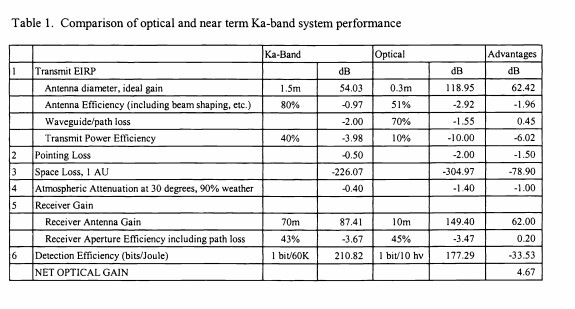
\includegraphics[width=1\columnwidth]{figures/laser-communication/bh3.jpg}
\caption{Comparison of optical and ka-band system performance}
\end{center}
\end{figure}
\noindent
Shown in Table 1 is the performance comparison between the proposed optical link and a near-term achievable RF link performance using Ka-band \cite{comparison}. Assuming equal power for the receiver and for monitor and control functions, the comparison is based on a constant DC power consumption by the transmit power amplifier. The optical link estimate is based on a 30 cm aperture diameter transmitter and a 1O m diameter receiver using 256-ary PPM and a I .06 jtm diode-pumped solid state laser. The Ka-band performance projection is based on the assumption that continuing improvements in Ka-band will lead to 
(a) implementation of Ka-band reception capability on the 70 m stations,
 (b) improved receiver aperture efficiency with either
the array feed or adjustable mirror technology, 
(c) improved spacecraft Ka-band transmitter power efficiency with high efficiency TWTAs, 
(d) Improved transmit aperture efficiency using off axis or displaced-axis antenna.

\subsubsection{Weather}

Despite of many such technological development, the major limitation of free-space laser communication (lasercom) performance is the atmosphere.  Atmospheric condition ultimately determines the laser communications systems pe for uplink-downlink , because a portion of the atmospheric path always includes turbulence and multiple scattering effects.
Heavy fog is a major weather constraint that almost completely blocks sources of light. Thus, it threatens FSO (Free-space optical communication) links by attenuating the light signal and almost breaking it.
 Light can be absorbed into the atmosphere. The phenomenon of absorption is caused mainly by the presence of water vapor and carbon dioxide in the air. These gases in addition to other types create what is called transmission windows that limit the passage of some light frequencies. The frequencies of laser sources are not in the range of absorption by these transmission windows, resulting in no effect on the communications link. laser sources are not affected by the atmospheric absorption of light during the transmission and receiving process.
Scattering is more of a concern to FSO links than absorption. This is true because scattering is a function of the light wavelength and the quantity and size of scattering elements in the atmosphere. scatter FSO light sources but the effect is considered negligible. The main weather contributor to signal attenuation is fog. Fog occurs when humidity of the air reaches a certain saturation level which condensates vapor to water droplets of microns of radius. These droplets are the major cause of scattering for infrared light. Even though fog droplets are smaller on average than cloud droplets but are huge when compared to the wavelength of the light.
The method of transmitting data from JIMO back to Earth is to use a free-space laser communications link from JIMO to an Earth-orbiting relay satellite. Using an optical receiver on an Earth-orbiting relay satellite is advantageous because it makes it possible to overcome the severe  atmospheric losses that may be experienced in direct optical transmission to a ground-based receiver.

\subsubsection{Proposed laser communication between Europa and earth}

The method of transmitting data from JIMO back to Earth is to use a free-space laser communications link from JIMO to an Earth-orbiting relay satellite. Using an optical receiver on an Earth-orbiting relay satellite is advantageous because it makes it possible to overcome the severe  atmospheric losses that may be experienced in direct optical transmission to a ground-based receiver. High data transmission rates can be achieved by using Wavelength Division Multiplexing (WDM) with multiple optical carriers each at different wavelengths. Additionally, a single transmitting telescope on JIMO can support the transmission of an optical beam that optically combines or multiplexes the data-modulated outputs from a multiple number of laser transmitters, each operating at different wavelengths.

Transmit optical aperture diameters ranging from 30 cm to 90 cm are evaluated. A single receiving telescope on the Earth-orbiting relay satellite is required with an optical aperture size that must be large enough to collect a sufficient amount of propagated light from the arriving optical light beam for carrying out reliable data demodulation and decoding. Receive optical apertures of 2.4 m and 3.6 m \cite{lasercom} .

\subsubsection{Wavelength}

Selection of wavelengths for optical communications depends on an understanding of the propagation channel, both through free space and atmosphere, and on the availability of components and subsystems including lasers, detectors, and optics. Additionally, issues pertaining to availability and reliability of components, especially lasers and detectors for user spacecraft, are critical to the selection of a viable communications wavelength. Considerations of missions and operational issues can also profoundly affect the choice of wavelength. Free space propagation loss decreases with wavelength, and provides the single most compelling reason to choose shorter wavelengths for laser communications. The angular beam diameter for a diffraction limited beam as measured by the first Airy disk of the diffraction pattern for a circular aperture is given by 2.44 $\tfrac{\lambda}{D}$, where D is the diameter of the transmitting aperture and $\lambda$ is the wavelength. Energy density at the receiver is inversely proportional to the square of the beam diameter. For a given distance z and transmitting aperture, the received energy density increases as $\lambda^{-2}$ below Fig., shows that the energy density decreased by three orders of magnitude as the wavelength increases from 0.4 to 12.5 micro m. This provides a strong argument to choose shorter wavelengths for laser communications \cite{article:wavelength}.
\begin{figure}[htb]
\begin{center}
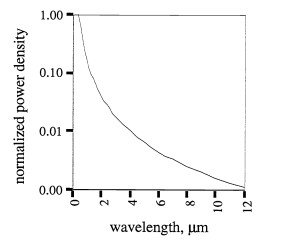
\includegraphics[width=0.7\columnwidth]{figures/laser-communication/bh4.jpg}
\caption{wavelength and power density}
\end{center}
\end{figure}
\\
We propose to use wavelengths on the ITU (International Telecommunication Union) grid specified for terrestrial fiber networks in the C band with nominal wavelengths between 1.53 and 1.57 microns (5 THz bandwidth). This choice of wavelengths takes advantage of the extensive terrestrial fiber network WDM technology currently available, including laser sources, photodiode detectors, erbium-doped fiber amplifiers (EDFA) for optical amplification, and WDM multiplexers and demultiplexers. 

\subsubsection{Modulation Type}

The large geometric space loss for communicating with deep space optical missions such as JIMO requires power efficient communication techniques.
optical detection receiver, is proposed to provide a highly power-efficient high data transmission rate system with reasonable implementation complexity. Specifically, a 256-slot PPM modulation scheme with RZ pulse shaping is considered, where each symbol carries 8 bits, requiring a 32-fold bandwidth expansion relative to the conventional binary on/off keying modulation normally employed in terrestrial fiber networks.

\subsubsection{Laser Source}

A high-power laser source at each wavelength can be implemented using a conventional laser diode followed by an EDFA power amplifier to produce 5 watts of launch power. Link closure at a 1.55-micron wavelength is then achieved for a 2.4 m receive aperture at data rates ranging from 2.5 Mbps for a 30 cm transmit aperture to 25 Mbps for a 90 cm transmit aperture. Increasing the receive aperture to 3.6 m increases the corresponding data transmission rates.

\subsubsection{Tx and Rx Aperture}

A single receiving telescope on the Earth-orbiting relay satellite is required with an optical aperture size that must be large enough to collect a sufficient amount of propagated light ,As we can see, the total telemetry data rate increased by increasing the transmitter aperture and receiver aperture, and adding more laser diode will increase the data rate. 
\begin{figure}[htb]
\begin{center}
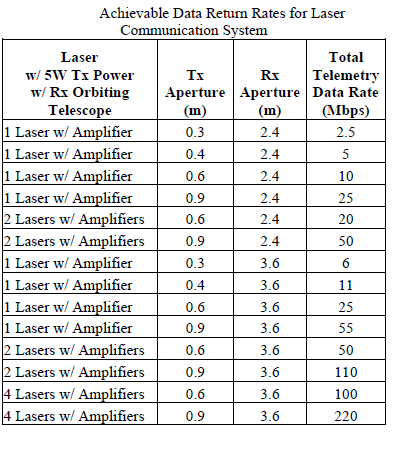
\includegraphics[width=0.7\columnwidth]{figures/laser-communication/bh5.png}
\caption{Achievable Data Return for laser Communication System}
\end{center}
\end{figure}
\\

\subsubsection{Pointing system}

Due to high data rates and reliability, the stability of the laser beam pointing is still a key technique which needs to be solved; otherwise, the beam pointing jitter noise would reduce the communication quality or, even worse, would make the inter-satellite laser communication impossible. 

\subsubsection{Weight, size, and power requirements}

The weight, size, and power requirements for a JIMO transmitter employing two wavelengths are estimated using extrapolation from previous work performed at The Aerospace Corporation.
\begin{figure}[htb]
\begin{center}
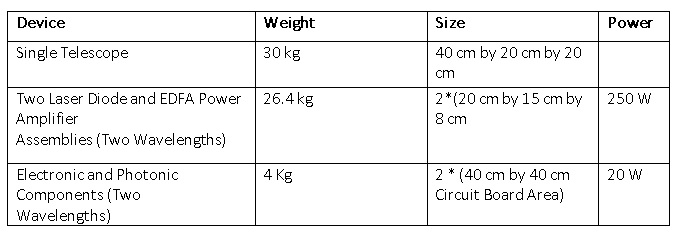
\includegraphics[width=1\columnwidth]{figures/laser-communication/bh11.jpg}
\caption{weight, size, and power requirements}
\end{center}
\end{figure}
\\

\subsubsection{Mission and Coverage limitation}

For almost all deep space missions, the mission profile will impose limits on spacecraft attitude and pointing of spacecraft during certain mission phases. Examples of such mission phases are the launch phase or inner cruise phase where spacecraft attitude is constrained by the trajectory or thermal consideration.there will be coverage holes that can potentially limit the mission planning.
-Difficulty in maintaining link with degraded spacecraft performance: This can include degraded station-keeping capability, degraded star tracker performance, or loss of time reference, will lead to unmanageable acquisition time.

The detection sensitivity is significantly worse at optical frequency, even with the use of high order PPM modulation . The optical receiver sensitivity can further degrade to 20-30 photons/bit under daytime conditions with current receiver technology.

Due to a high distance and difficulty of continuous acquisition and tracking, we can not use laser communication for this mission.


\autsection{Surface-to-Orbiter}{Rasmus Lundby Pedersen}
As it was discussed in the section covering the initial considerations, it was decided that using the orbiting satellite as a relay-station, in stead of transmitting data directly to and from earth to Europa, was the only viable solution for the collective communication systems design.\\
This section will focus on the considerations concerning the design of the antenna system, the losses tied to the system and the surrounding environment, limitations, and required power for the data transfer between the surface of Europa and the satellite.

\subsection{Considerations and General Assumptions}
There are several critical considerations tied to the design of a communication link between two antennas. For space applications, these generally include, but are not necessarily limited to:

\begin{itemize}
\item \underline{Transmission distances and relative loaction.} A critical parameter of the design is the distance that the transmitted data signal must travel between a transmitter and a receiver. This aspect governs part of the required power usage (and in turn, the antennas' gains), while a target antenna moving with reference to the transmitting antenna may require tracking capabilities to be installed. Of course, the last point will depend on the available power and gain of the antennas.
\item \underline{Atmospheric Environment.} Losses in the systems varies greatly with the environment in which the transmitted signal must travel. Electromagnetic waves will always see losses when travelling in free-space, or at least near-vacuum, but will be significantly attenuated if for example they are travelling in a thick atmosphere like our Earth's.
\item \underline{Structural restrictions.} Ground-based antennas usually have very few space-restrictions, and can often thus be very large. However, when designing a system for a satellite, or an extraterrestrial exploration mission, the volume and mass of the product must be kept as an absolute low. Larger antennas are in some cases synonymous with higher gain (See parabolic antennas), so there will often be a trade-off here.
\end{itemize}

Smaller, more specific aspects should also be included in the considerations, such as the size of the transmit windows as well as the bit-rate of the transmitted data.\\\\
We currently believe Europa has an almost negligible tenuous oxygen atmosphere, which is a major advantage in the power-calculations in the final link-budget \cite{SciStrat}. Further studies of the Jovian satellite, and additional mission, like the planned CLIPPER, are required to support this theory, but it means that we can assume an signal attenuation of about $\alpha_{atmos}=2\,\mathrm{dB}$ in the atmosphere.\\
\\
The moon is constantly victim to extreme amounts of radiation from Jupiter, which is estimated to be 10 times stronger than Earth's Van Allen belts CITE. One consequence of this is, that any electronics parked in a region illuminating by this radiation would be destroyed immediately. Another, is the massive radiation noise picked up by the antennas, which would effectively render the communication link useless.\\ 
We're fairly certain Europa is tidal locked to Jupiter, which means that roughly the same side of the moon points toward the planet at all times, with a small derivation through time. The feature will likely be utilized by landing the penetrator module on the anti-Jovian side of the moon. This way, the comm-link will constantly be shielded by the moon itself, and the radiation noise from Jupiter can be neglected. An article written by 3 undergraduate students from the University of Texas state that they would expect to transmit through a Jovian radio noise of $T_{ant}=2000\,\mathrm{K}$ \cite{DORRA}, in the S-band. However, it is unsure if they intend to operate on the anti- or pro-Jovian side of the moon, and we're not sure where they have obtained the noise temperature number from.\\
\\
We expect the round-trip time of the relaying satellite's orbit around Jupiter to be around 13 Earth days. During those 13 days, data from the instrument suite will be transmitted from the penetrator to the surface module and stored in a memory-block located in the part of the descent vehicle that had been submerged a few meters in the surface-ice, for radiation protection.\\
\\
It's fairly common for satellites to carry complimentary X- and S-band\footnote{The X-band ranges from 8-12 $GHz$, and the S-band ranges from }, low- and high-gain antennas for near-Earth passes and deeper space communications respectively\footnote{A S-band telemetry transmitter is used for the communication to Earth, in the CLIPPER mission.}. In an effort to re-use some of the instruments on the satellite, the X-band low-gain amplifier will be utilized for the Surface-to-Orbiter link. This locks the carrier frequency to $f_c=8-12\,\mathrm{GHz}$, and thus the free-space signal wavelength to $\lambda_0=\frac{c}{f_c}=25-37mm$, where c is the speed of light, and will most likely govern the size of the antenna, depending on the design.
\subsection{Drivers}
We determined that the bottle-neck of the communication chain between the penetrator and Earth would lie in the thru-ice link, with it bit-rate limited at 10kbps. With a orbital round trip for the satellite of 13 days, this means that we need to transmit a data load of around $13\,\mathrm{days}\cdot 10\, \mathrm{\frac{kb}{s}}=11\,\mathrm{Gb}$ in 3 hours; an average bit-rate of $b=\frac{11\mathrm{Gb}}{3\mathrm{h}}=1\,\mathrm{\frac{Mb}{s}}$.\\
However, it may prove that the bottleneck is that this link, since the bit-rate of transmitted signal is directly proportional to the required transmitting power.\\
\\
A loose assumption was made, that the transmission window starts when the satellite is located $45^\circ$ above the horizon, when the distance between the surface module and the orbiter is around 6600km. This is the absolute worst-case scenario, since the actual distance will be much lower in the majority of the time in the transmission window. The link budget is calculated for this distance in order to be sure that we can guarantee a certain standard of signal quality.
\subsection{Solution Proposals}
In this part, three solution proposals are presented, and the most suitable decided. The three chosen designs are:
\begin{itemize}
\item The parabolic antenna.
\item Phased array patch antenna.
\item Crossed dipole antenna. 
\end{itemize}
Design and production costs are not considered for the three solutions. 
\subsubsection{Parabolic Antenna}
The parabolic antennas are typically used for ground station antennas and on satellites with well-known and reliable attitude orientation, with respect to its target.\\
A main advantage is it's considerable antenna gain, which is given by:
\begin{equation}
G = \eta_a\left(\frac{\pi D}{\lambda}\right)
\end{equation}  
Where $\eta_a$ is the aperture efficiency, typically ranging between $0.55<\eta_a<0.7$, D is the circular diameter of the parabolic dish and $\lambda$ is the signal wavelength.\\
It can be seen that the gain of the antenna is directly proportional to its size, which itself is independent of the signal's wavelength. This means that the antenna can be scaled for the desired gain, within structural limitations.\\
\\
A disadvantage of a high-gain antenna is, that must be oriented towards its target with fairly high accuracy. This can be achieved by mechanically tracking the target on the sky with motors, which in itself is un-desired for any space-related mission. Pin-pointing the target also proves difficult for a surface based station on Europa, where we are without a network of GPS satellites to track the position of the surface antenna with respect to the orbiting satellite. We have practically no way of knowing where to point the antenna, and the benefits of its large gain will be lost. 
\subsubsection{Phased-Array patch Antenna}
The problem of using mechanical tracing for the parabolic antenna can be solved by using phased-array patch-antennas in stead. A single flat patch antenna doesn't necessarily come with a particularly impressive antenna gain, but an array of the has shown to enable us to modify its radiation pattern. Differentiating the phases between the patches will in turn make it possible to direct the radiation pattern dynamically, and the high carrier frequency allows us to reduce the size of the patch antenna significantly compared to the parabolic antenna. the principle of a phased-array antenna is shown on figure \ref{fig:phased}\footnote{\url{http://tempest.das.ucdavis.edu/mmwave/paa_files/image005.png}}.\\
\begin{figure}[htb]
	\centering
	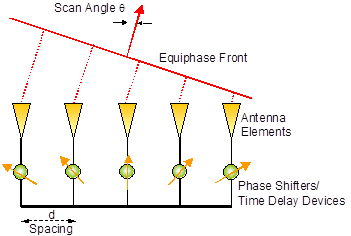
\includegraphics[width=0.75\textwidth]{figures/Rasmus/phased}
	\caption{A simplified concept illustration of the Phased array antenna .
	\label{fig:phased}}
\end{figure}
However, the issue of tracking the target on the sky still persists and remains un-solved. Therefore, it seems that the parabolic antenna and the 
\subsubsection{Crossed Dipole Antenna}
\begin{figure}[htb]
	\centering
	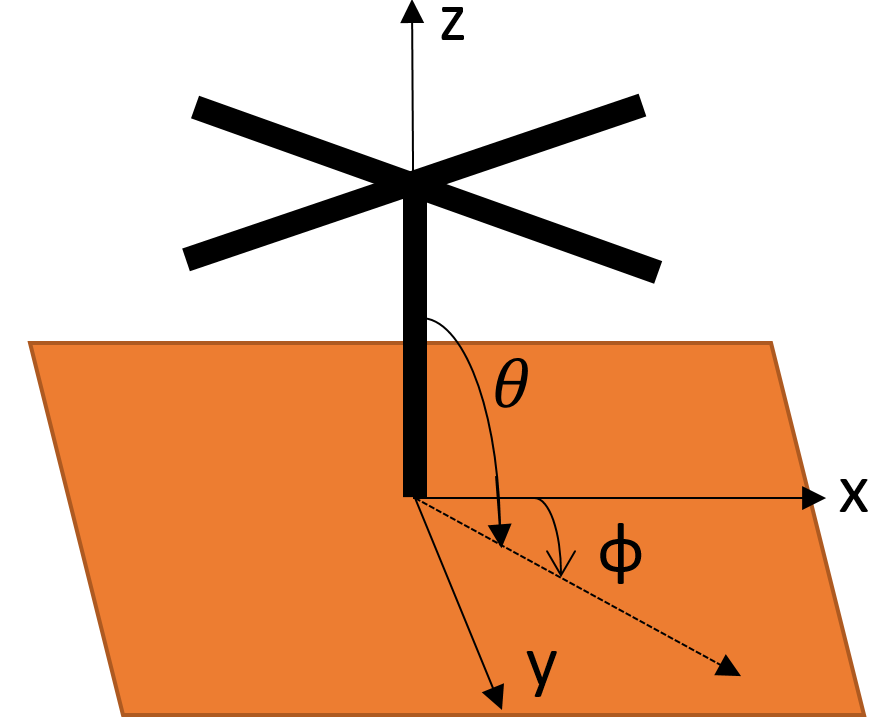
\includegraphics[width=0.6\textwidth]{figures/Rasmus/CrossDip}
	\caption{Crossed half-wave dipole antenna drawing.
	\label{fig:DrossDip}}
\end{figure}
\begin{figure}[htb]
	\centering
	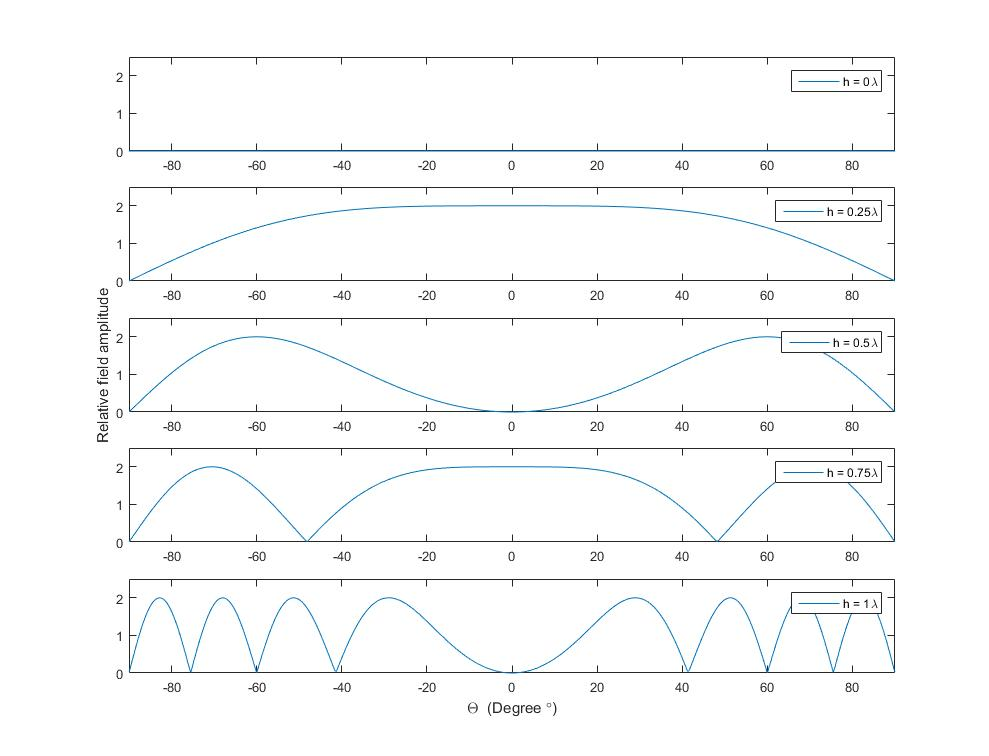
\includegraphics[width=0.75\textwidth]{figures/Rasmus/Lopes}
	\caption{Theta-variant of the radiation pattern for the crossed half-wave dipole antenna.
	\label{fig:Lopes}}
\end{figure}
\subsection{Implementation and Link budget}

\iffalse
1. Introduction and considerations for the link
      * (Orbit characteristics and Europa Environment)
1. Link Drivers
   1. Radiation (Europa surf dead zone)
   2. Low Power
   3. Transmission Relay Window
      * Dataload
      * Bitrate
   1. Low Temperature Operation
   2. Line of Sight (viewing angles)
      * Communication while descent maneuver
      * Antenna choice
      * Mechanical stabilizers
1. Link Budget
2. Solution Proposal
3. Drivers to other systems
\fi